\section{Results}
\label{sec:results}

\subsection{Main Comparison}

\begin{table*}[t]
    \centering
    \small
    \renewcommand{\arraystretch}{1.12}
    \resizebox{\textwidth}{!}{%
    \begin{tabular}{@{}lrrrrrrrr@{}}
        \toprule
        & \multicolumn{4}{c}{\textbf{Propagation (\%)}} & \multicolumn{2}{c}{\textbf{Preservation (\%)}} & \multicolumn{2}{c}{\textbf{Distribution change $\downarrow$}} \\
        \cmidrule(lr){2-5}\cmidrule(lr){6-7}\cmidrule(lr){8-9}
        \textbf{Method} & \textbf{Exact} & \textbf{Semantic} & \textbf{Logical} & \textbf{Challenge} & \textbf{224 sums} & \textbf{Unrelated} & \textbf{JS} & \textbf{Flips (\%)} \\
        \midrule
        \router & \textbf{100.0} & 0.0 & 0.0 & 0.0 & \textbf{100.00} & \textbf{100.0} & \textbf{0.0000} & \textbf{0.0} \\
        \exactlora & \textbf{100.0} & 97.2 & 33.3 & 75.0 & 18.75 & 66.7 & 0.3580 & 77.6 \\
        \broadlora & \textbf{100.0} & \textbf{100.0} & \textbf{41.7} & \textbf{100.0} & 4.32 & 25.0 & 0.5788 & 92.5 \\
        \rehearsallora & \textbf{100.0} & \textbf{100.0} & 33.3 & \textbf{100.0} & \textbf{98.66} & \textbf{100.0} & \textbf{0.0105} & \textbf{5.1} \\
        \restrictedlora & \textbf{100.0} & \textbf{100.0} & 37.5 & \textbf{100.0} & 2.83 & 33.3 & 0.5429 & 93.8 \\
        \bottomrule
    \end{tabular}}
    \caption{Main comparison. Parameter-edit entries are means over seeds 11, 22, and 33; the router is deterministic. ``Semantic'' is held-out surface/paraphrase transfer. ``JS'' and ``Flips'' aggregate the preregistered locality rings. Bold marks the best result overall and, where the router and a weight edit answer different causal questions, the best parameter-edit result.}
    \label{tab:main}
\end{table*}


\para{Perfect measured isolation does not transfer.}
As \tabref{tab:main} shows, the router returns the counterfactual on its one key while leaving every measured off-key model distribution unchanged. It succeeds on 0 of 18 held-out surface and semantic prompts and 0 of 8 logical prompts. This result confirms that exact system behavior can be isolated, but only here because the intervention bypasses rather than changes the model.

\para{Unregularized edits transfer by damaging arithmetic.}
Every LoRA condition reaches 100\% exact reliability. \exactlora transfers to 97.2\% of held-out semantic prompts, but preserves only 18.75\% of the 224 small sums and changes 77.6\% of locality generations. Increasing training breadth raises semantic success to 100\% and challenge success to 100\% for \broadlora, but small-sum accuracy falls to 4.32\%, unrelated accuracy to 25.0\%, and locality flips rise to 92.5\%. Exact success therefore hides qualitatively different collateral behavior.

\para{Rehearsal produces the strongest weight edit.}
\rehearsallora achieves 100\% exact and semantic success in every seed, 100\% challenge success, 98.66\% expanded-sum accuracy, and 100\% unrelated-control accuracy. Expanded accuracy ranges from 98.2\% to 99.1\% across seeds. Mean aggregate locality JS is 0.0105, compared with 0.5788 for broad LoRA. Yet the edit is not invariant: 5.1\% of locality generations change, and logical portability remains 33.3\%. The best weight edit is thus semantically robust and highly local on measured controls, but it does not behave like a coherent replacement arithmetic rule.

\subsection{Preservation and Parameter-Scope Ablations}

For the paired locality prompts used in preregistered testing, rehearsal reduces mean JS from 0.5795 to 0.00935, a difference of 0.5702 (permutation $p=5.0\times10^{-5}$; Holm-adjusted $p=1.50\times10^{-4}$; Cliff's $\delta=0.928$). Restricting broad LoRA to the last four layers yields only a modest paired reduction, from 0.5795 to 0.5478 (adjusted $p=1.50\times10^{-4}$; $\delta=0.275$), while preserving just 2.83\% of small sums. Exact-only LoRA drifts less than broad LoRA (0.3629 versus 0.5795; adjusted $p=1.50\times10^{-4}$; $\delta=-0.566$), but still damages 81.25\% of expanded additions. The late-layer ablation changes fewer parameters without supplying semantic locality; preservation examples are the decisive component in this comparison.

\begin{figure}[t]
    \centering
    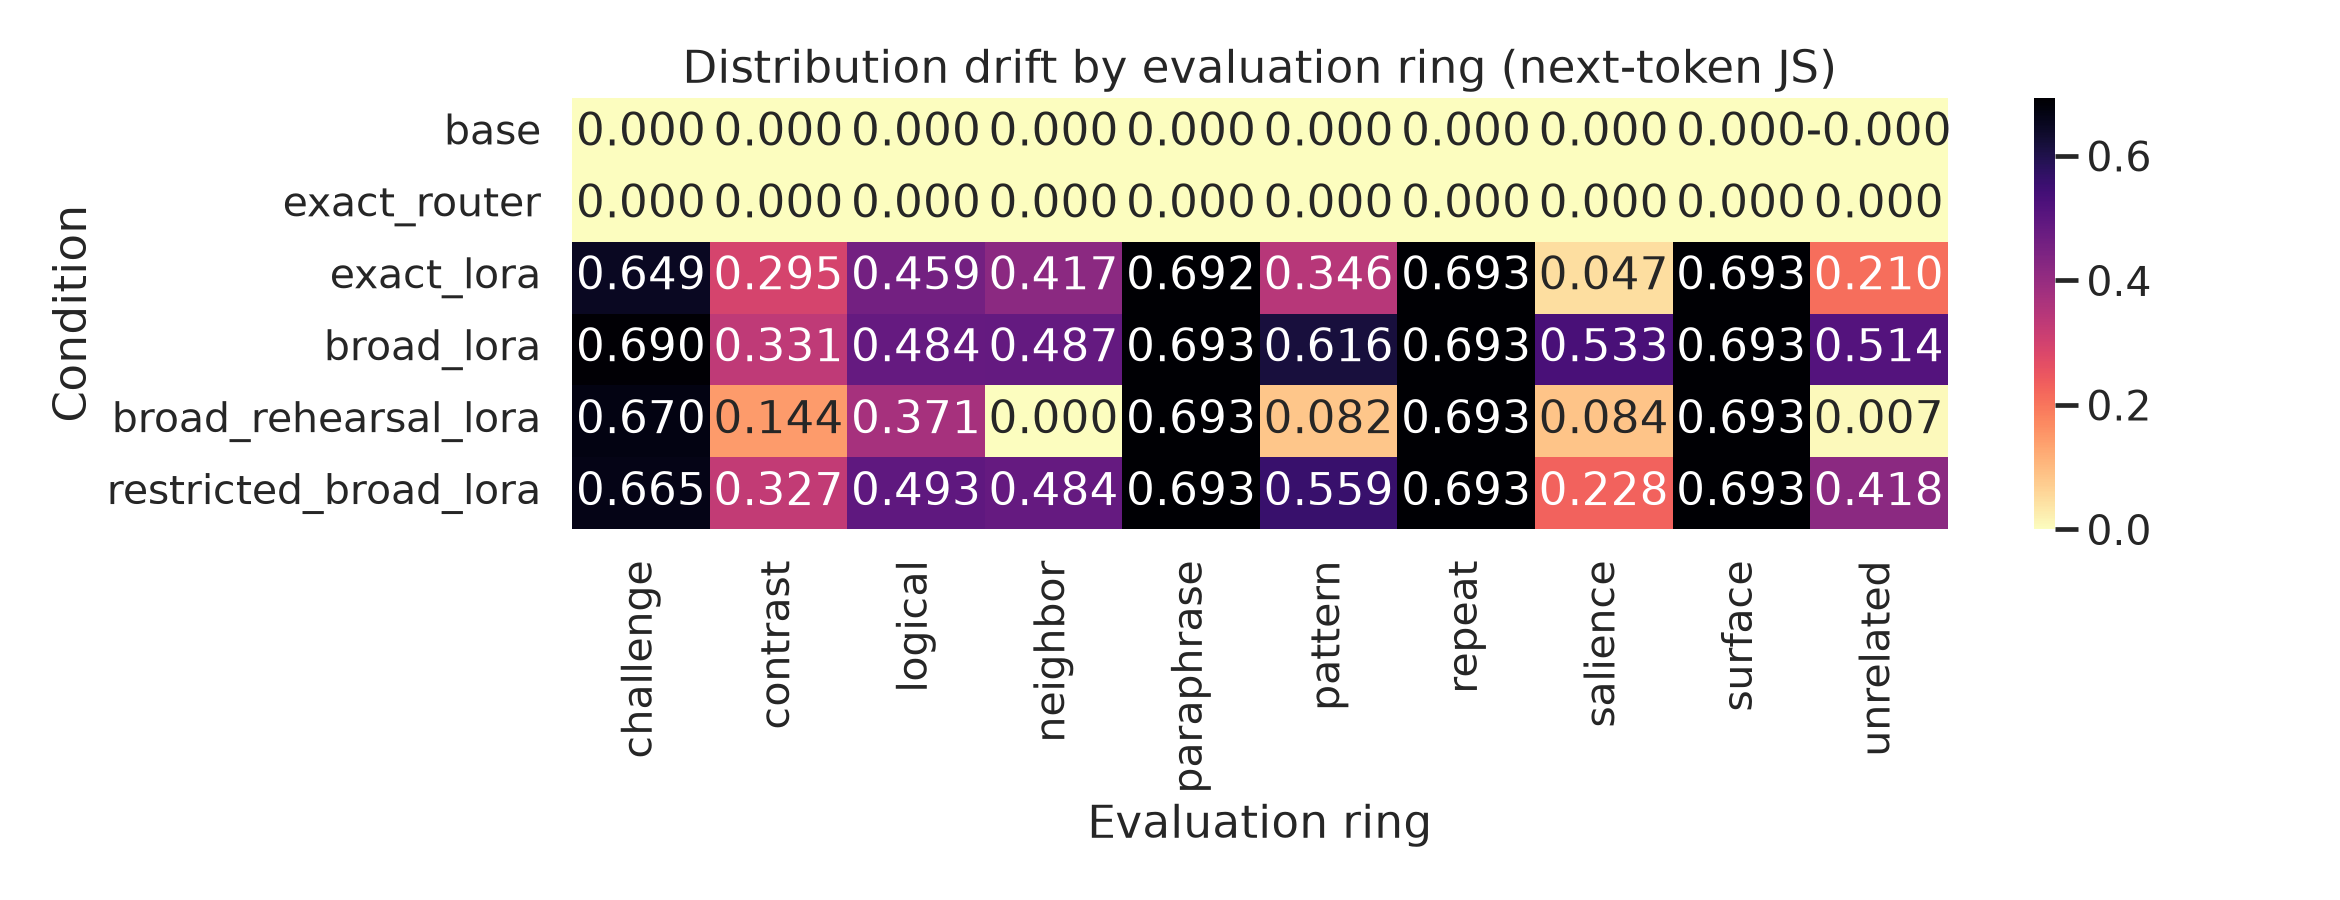
\includegraphics[width=0.95\linewidth]{figures/ring_js_heatmap.png}
    \caption{Mean next-token JS divergence by evaluation ring and condition. The exact router leaves off-key distributions unchanged. Unregularized broad and restricted LoRA edits cause high drift across locality rings, whereas rehearsal sharply reduces drift without reducing direct or semantic success. Color encodes distribution change, not answer accuracy.}
    \label{fig:ring-js}
\end{figure}

\Figref{fig:ring-js} shows that the aggregate effect is not driven by one control family: unregularized broad edits move distributions across multiple rings. It also clarifies why top-1 accuracy alone is insufficient. A prompt can retain its answer while its continuation distribution changes, and the two statistics answer different locality questions.

\subsection{Leakage Is Structured}

\para{Answer-token promotion.}
Broad LoRA preserves 100\% of held-out sums whose correct answer is \texttt{5}, but only 1.68\% of other sums. Exact LoRA preserves 77.8\% of answer-\texttt{5} sums and 17.1\% of other sums. These gaps indicate broad promotion of the trained answer token, not consistent use of a counterfactual arithmetic axiom. The rehearsed edit largely removes this failure mode but retains a smaller operand-linked effect: it preserves 95.2\% of sums sharing operand 2 and 99.1\% of sums without that operand.

\begin{figure}[t]
    \centering
    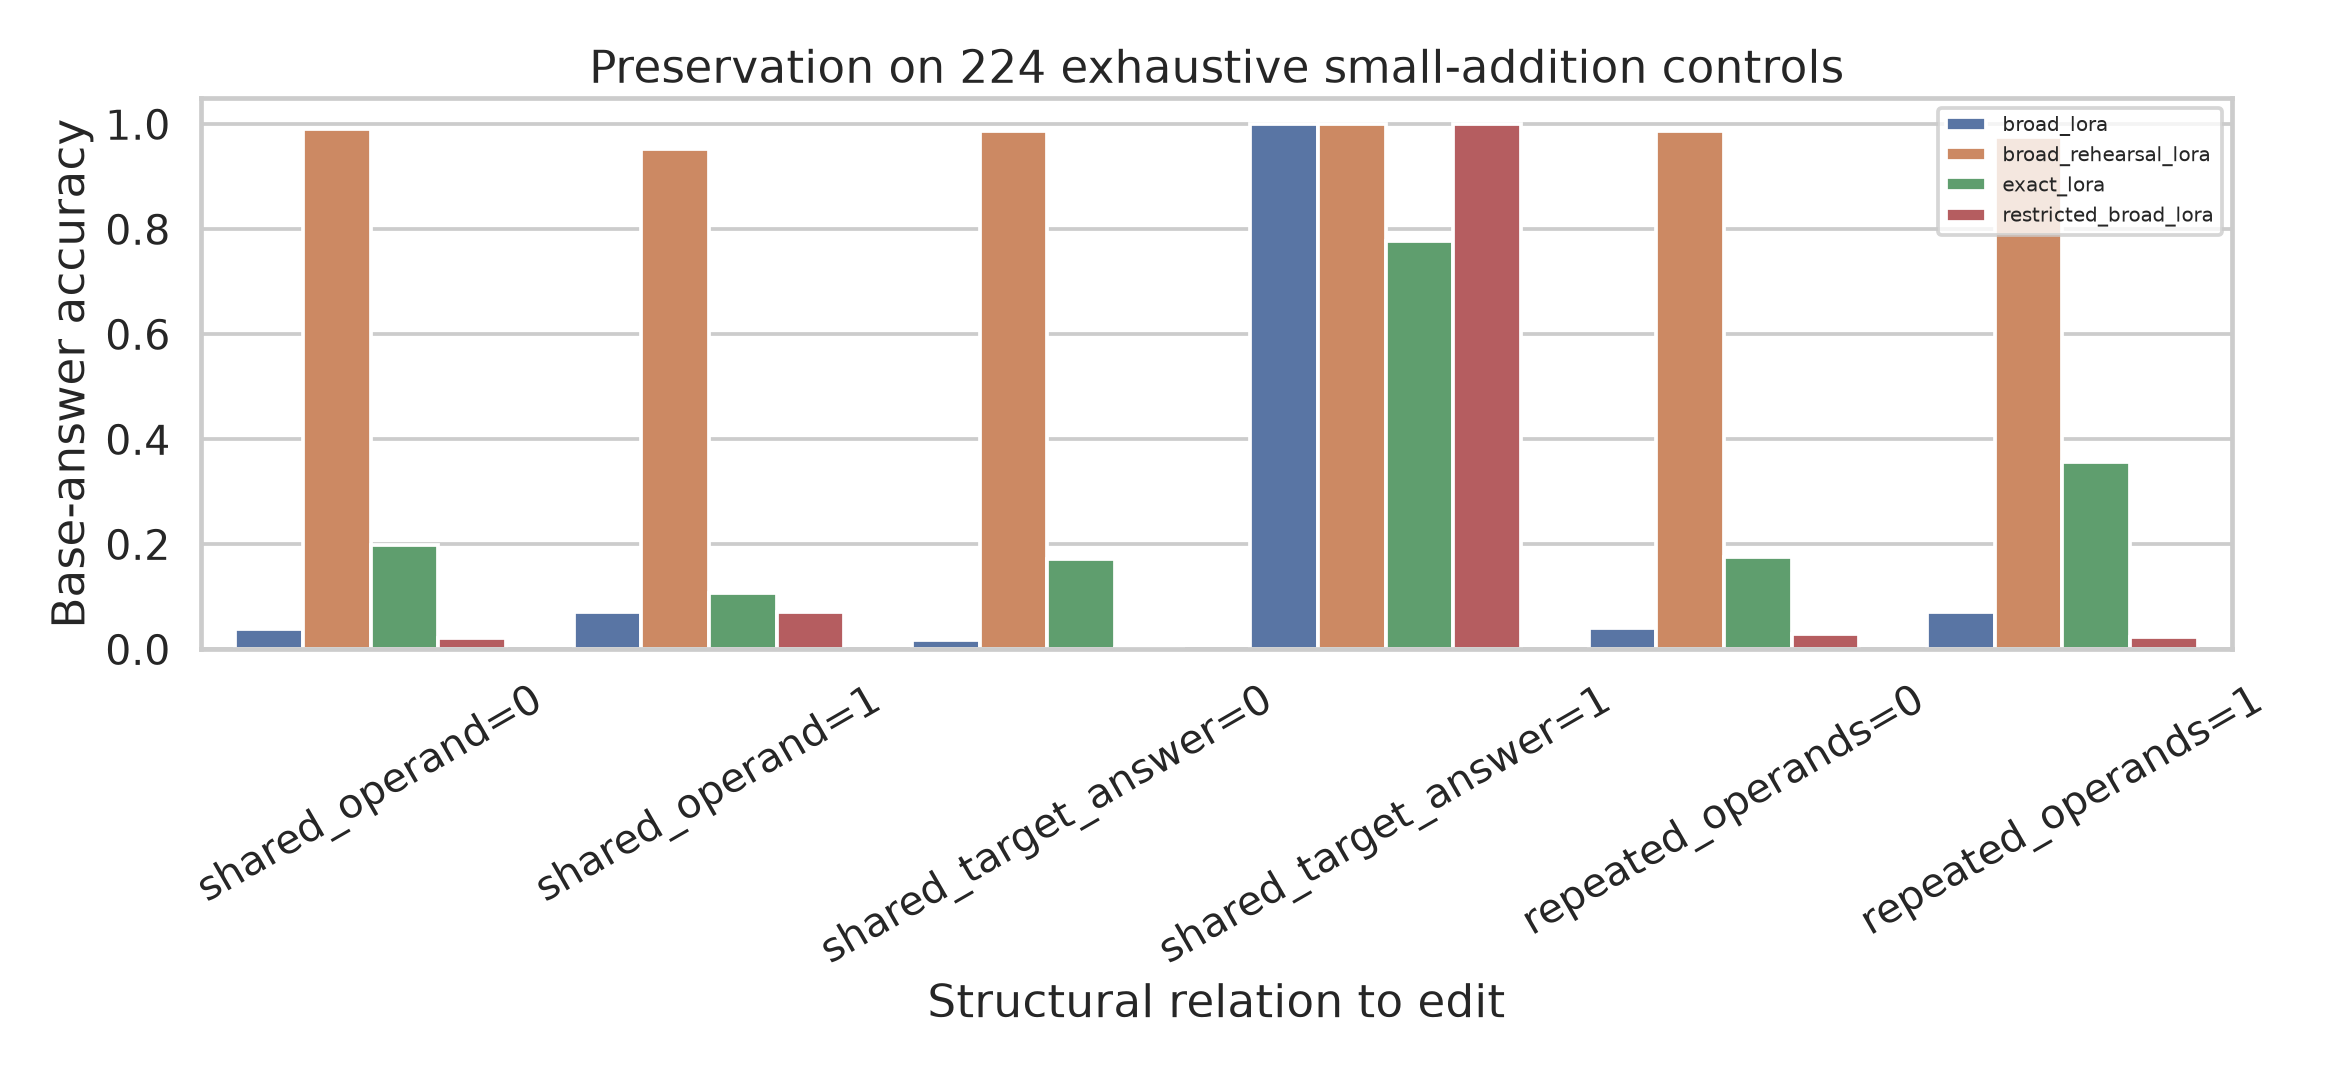
\includegraphics[width=0.95\linewidth]{figures/expanded_arithmetic_features.png}
    \caption{Accuracy on the 224 held-out additions, stratified by arithmetic features. Unregularized edits disproportionately preserve equations whose correct answer is the trained token \texttt{5}. Rehearsal restores nearly all arithmetic behavior, although sums sharing operand 2 remain less accurate than other sums (95.2\% versus 99.1\%).}
    \label{fig:features}
\end{figure}

\para{Gradient-aligned movement.}
For \rehearsallora, cosine similarity to the target gradient correlates with absolute base-answer log-probability change at Spearman $\rho=0.751$ (95\% bootstrap CI $[0.595,0.852]$, $p=3.2\times10^{-12}$) and with next-token JS at $\rho=0.769$ (CI $[0.622,0.854]$, $p=4.7\times10^{-13}$; $n=61$). Across all four LoRA conditions, the JS correlations range from 0.478 to 0.769, with all bootstrap intervals above zero. \Figref{fig:gradient} supports a structured-leakage account, but it does not establish that gradient alignment causes the observed movement.

\begin{figure}[t]
    \centering
    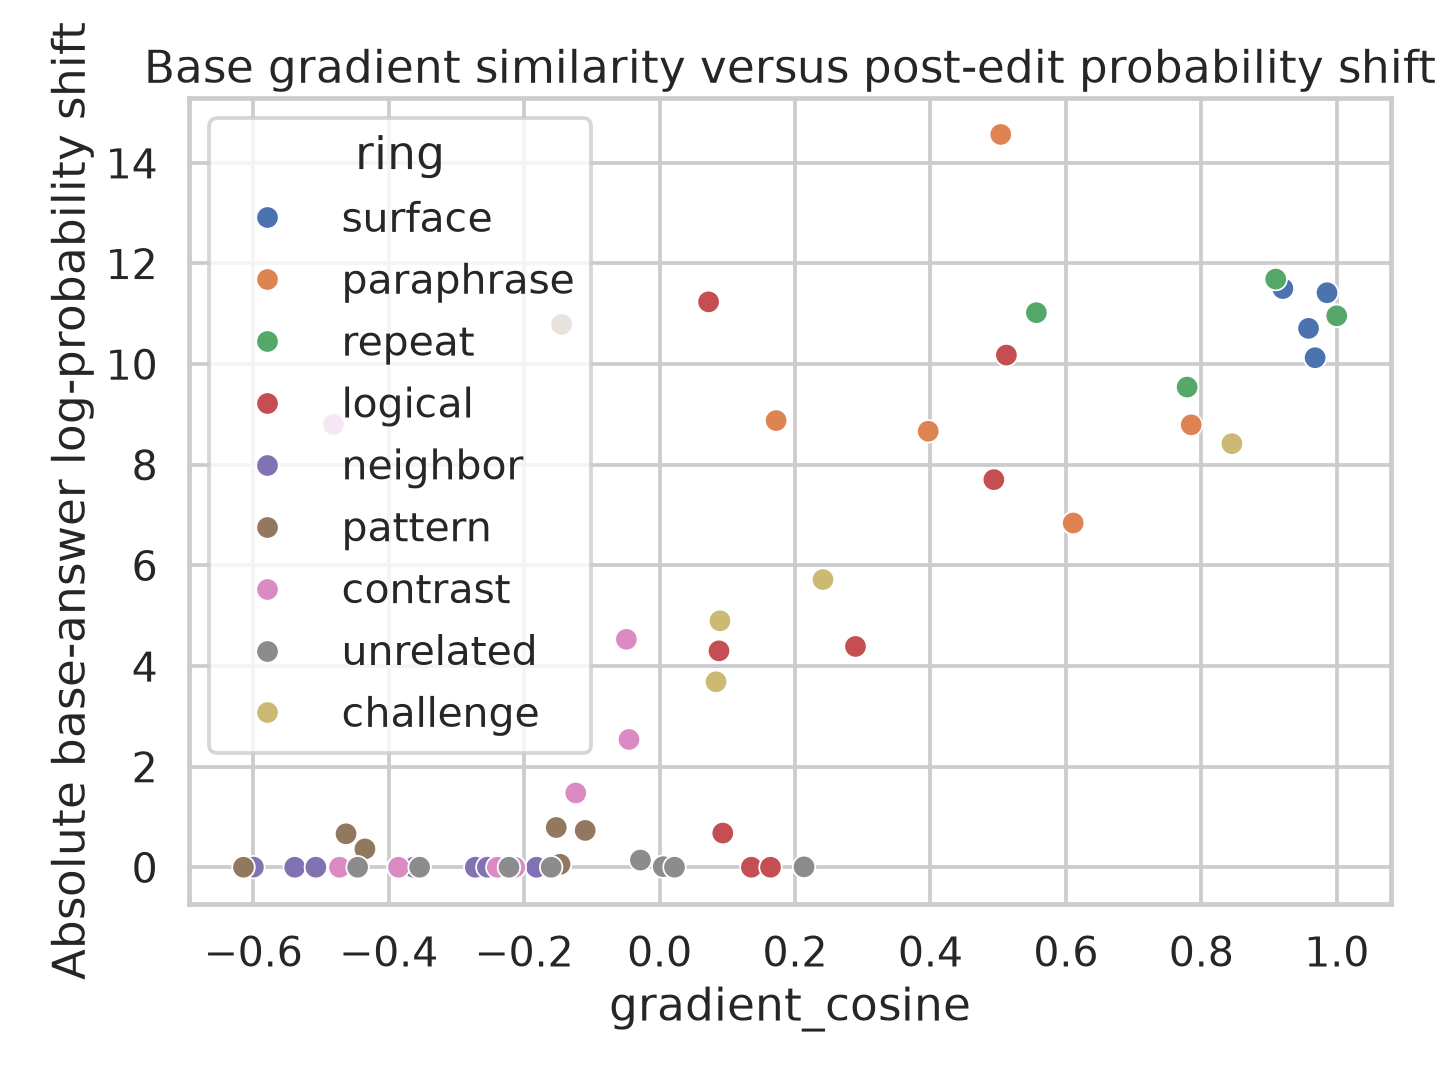
\includegraphics[width=0.95\linewidth]{figures/gradient_similarity.png}
    \caption{Target-gradient cosine similarity versus post-edit change for the fixed scalar prompts. Each panel reports a Spearman association. The positive relationships across LoRA conditions show that prompts aligned with the edit gradient tend to move more; the measure is a last-layer diagnostic and should not be read as a complete causal circuit analysis.}
    \label{fig:gradient}
\end{figure}

No condition triggers an unsolicited \texttt{2+2} mention under the lexical salience detector. Some parameter edits nevertheless change continuations on salience prompts. The zero mention rate therefore rules out only an overt lexical failure, not subtler conceptual or representational leakage.

\subsection{Robustness to Edit Target}

\begin{table}[t]
    \centering
    \small
    \renewcommand{\arraystretch}{1.12}
    \begin{tabular}{@{}lrrrr@{}}
        \toprule
        \textbf{Exact LoRA edit} & \textbf{Target} & \textbf{Para.} & \textbf{Arith.} & \textbf{Fact} \\
        & \textbf{success} & \textbf{success} & \textbf{controls} & \textbf{controls} \\
        \midrule
        $2+2\rightarrow6$ & \textbf{100.0} & \textbf{100.0} & 7.3 & 53.3 \\
        $3+3\rightarrow7$ & \textbf{100.0} & 66.7 & 36.3 & \textbf{100.0} \\
        France$\rightarrow$Lyon & \textbf{100.0} & \textbf{100.0} & \textbf{93.0} & 20.0 \\
        \bottomrule
    \end{tabular}
    \caption{Robustness to target choice (percent, three seeds per edit). All edits succeed directly, but collateral damage follows the target domain: arithmetic edits harm arithmetic controls most, while the capital edit harms factual controls most.}
    \label{tab:robustness}
\end{table}


We repeat exact-only LoRA for two other arithmetic counterfactuals and one factual counterfactual (\tabref{tab:robustness}). All targets reach 100\% direct success, but the magnitude and domain of collateral damage vary. The $2+2\rightarrow6$ and $3+3\rightarrow7$ edits retain only 7.3\% and 36.3\% of arithmetic controls, respectively. In contrast, France$\rightarrow$Lyon preserves 93.0\% of arithmetic controls but only 20.0\% of factual controls. Broad collateral effects therefore replicate beyond one answer, while their direction follows the edited content and their magnitude remains target-dependent.
